\documentclass[12pt, letterpaper]{article}
\usepackage[left=1.00in, right=1.00in, top=1.00in, bottom=1.00in]{geometry}
\usepackage{amsmath}
%\usepackage{apacite}
\usepackage{graphicx}

\title{Chapter 2}
\author{Daniel C. Furr}
\date{\today}


\begin{document}

\newcommand{\genupsilonsq}{0.11}
\newcommand{\gentau}{\{0.00, 0.10, 0.30, 0.50\}}
\newcommand{\gentausq}{\{0.00, 0.01, 0.09, 0.25\}}
\newcommand{\genrsq}{\{1.00, 0.92, 0.55, 0.30\}}

\newcommand{\comment}[1]{{\footnotesize[\textit{#1}]}}

\maketitle

\tableofcontents
\newpage
{\footnotesize }


\section{Introduction}


\section{Simulation and analysis methods}

\subsection{Data generation}

Data are simulated for varying numbers of persons ($P$) and items ($I$) using the model described in Chapter~1. Specifically, the composite item difficulties are generated as
\begin{equation}
	\delta_i = x_{1i}\beta_1 + x_{2i}\beta_2 + x_{3i}\beta_3 + x_{4i}\beta_4 + 
		x_{2i}x_{3i}\beta_5 + \epsilon_i
\end{equation}
\begin{equation}
	\epsilon_i \sim \mathrm{N}(0, \tau^2)
,\end{equation}
where $x_{1i} = 1$ is an intercept and $x_{2i}$, $x_{3i}$, and $x_{4i}$ are indicator variables which each equal 1 for half of the items and 0 for the remainder. Each possible combination of the indicators occurs an equal number of times, and the generating model includes one interaction, $x_{2i}x_{3i}$. Table~\ref{tab:X} provides the design matrix for item covariates. The rows of the design matrix are repeated to accommodate multiples of 8.

% matrix: X file: figs/table_x.tex  23 Oct 2015 12:20:52
\begin{table}[htbp]
\caption{\label{tab:X} Items design matrix}\centering\medskip
\begin{tabular}{ccccc} \hline \hline
$x_1$ & $x_2$  & $x_3$  & $x_4$  \\  \hline 
1 & 0 & 0 & 0 \\  
1 & 0 & 0 & 1 \\  
1 & 0 & 1 & 0 \\  
1 & 0 & 1 & 1 \\  
1 & 1 & 0 & 0 \\  
1 & 1 & 0 & 1 \\  
1 & 1 & 1 & 0 \\  
1 & 1 & 1 & 1 \\  
\hline \hline \end{tabular}
\end{table}


The composite abilities are generated as
\begin{equation} \label{eq:theta}
	\theta_p = w_{1p}\gamma_1 + w_{2p}\gamma_2  + \zeta_p
\end{equation}
\begin{equation} \label{eq:zeta}
	\zeta_p \sim \mathrm{N}(0, \sigma^2)
,\end{equation}
where $w_{1p}$ and $w_{2p}$ are also crossed indicator variables. Table~\ref{tab:W} presents the design matrix for person covariates, the rows of which are repeated to accommodate the $P = 4n$ persons.

% matrix: W file: figs/table_w.tex  23 Oct 2015 12:20:52
\begin{table}[htbp]
\caption{\label{tab:W} Persons design matrix}\centering\medskip
\begin{tabular}{cc} \hline \hline
$w_1$  & $w_2$  \\  \hline 
0 & 0 \\  
0 & 1 \\  
1 & 0 \\  
1 & 1 \\  
\hline \hline \end{tabular}
\end{table}


A key feature of the generated datasets (and data of this type more generally) is the extent to which the item covariates account for the composite item difficulties. To this end, let $\upsilon^2 = \mathrm{var}(x'\mathbf{\beta})$ represent the variance of the structural part of item difficulty. Because of the item design, $\upsilon^2$ does not vary between simulated datasets, even if they have differing numbers of items (so long as $I$ is a multiple of $8$.). The total item variance is $\upsilon^2 + \tau^2$. Then
\begin{equation}
R^2 = \frac{\upsilon^2}{\upsilon^2 + \tau^2}
\end{equation}
represents the proportion of item variance accounted for by the item predictors. 

The generating values for the structural part of item difficulties are $\beta = \{ -.5, .5, .5, .5, -.5 \}$ in all simulation conditions, and so $\upsilon^2 = \genupsilonsq$ in all conditions. Figure~\ref{fig:rsq-vs-tau} displays $R^2$ as a function of $\tau$ with $\upsilon^2$ fixed to this value. The points marked indicate the generating values of $\tau$, which are $\tau \in \{\gentau\}$ (or equivalently,  $\tau^2 \in \{\gentausq\}$). This choice yields $R^2 \in \{\rsq\}$. On the person side, the generating values are fixed across conditions, with $\gamma = \{ .5, .5 \}$ and $\sigma = 1$. The numbers of persons and items vary: $I \in \{32, 128\}$ and $P \in \{300, 1000\}$.

\begin{figure}[tbp]
	\centering
	\includegraphics[height=3in, trim = 1mm 1mm 1mm 1mm, clip=true]
		{chapter_2/figs/rsq_vs_tau.pdf}
	\caption{$R^2$ versus $\tau$ for the simulations. The points indicate generating values of $\tau$.}
	\label{fig:rsq-vs-tau}
\end{figure}

In summary, three factors are varied between simulation conditions in a crossed design: $\tau$ (and by extention, $R^2$), $I$, and $P$. All other elements are fixed across conditions. Because cross-validation features prominently in this chapter, multiple datasets are simulated within each replication. A ``training'' dataset is created as described above, and along with it three ``test'' datasets are formed: one representing a sample with new items (corresponding to new draws of $\epsilon_i$), one representing a sample with new persons (new draws of $\zeta_p$), and the last representing a sample with both new items and new persons.


\subsection{Models}

Three models, differing only in specification of $\delta_i$, are fit. Model 1 includes only the ``main effects'' for the item covariates:
\begin{equation}
\delta_i^{(1)} = x_{1i}\beta_1 + x_{2i}\beta_2 + x_{3i}\beta_3 + x_{4i}\beta_4
.\end{equation}
Model 2 adds an interaction:
\begin{equation}
\delta_i^{(2)} = x_{1i}\beta_1 + x_{2i}\beta_2 + x_{3i}\beta_3 + x_{4i}\beta_4
+ x_{2i}x_{3i}\beta_5
.\end{equation}
Model 3 adds an additional, extraneous interaction:
\begin{equation}
\delta_i^{(3)} = x_{1i}\beta_1 + x_{2i}\beta_2 + x_{3i}\beta_3 + x_{4i}\beta_4
+ x_{2i}x_{3i}\beta_5 + x_{3i}x_{4i}\beta_6
.\end{equation}
None of the analysis models includes the residual $\epsilon_i$. Each analysis model models ability as in Equations~\ref{eq:theta} and \ref{eq:zeta}. %When $\tau = 0$ is used to generate the data, Model 2 is the true model. Otherwise, none of three match the data generating model.


\section{Naive cross-validation methods}

One naive approach to model selection is the use of significance testing for parameters. In order to select among the three analysis models, a researcher may fit Model~2 and make a judgment based on the p-value for $\beta_5$, the parameter associated with the interaction. If non-significant, the researcher may select Model~1. Otherwise, the researcher may fit Model~3. If the additional interaction ($\beta_6$) is significant, Model~3 would be selected. Otherwise, Model~2 would be selected. This is a forward stepwise procedure.

%Figure~\ref{fig:pcheck-bar} presents the proportion of times each model was selected across conditions (combination of $I$, $P$, and $\tau$) when selection is performed via p-values. Within each condition, 200 replications are performed. This method works well when $\tau$ is small but poorly otherwise, and this trend is similar for all combinations of $P$ and $I$. 
This method works well when $\tau$ is small but poorly otherwise.
When $\tau = 0$, Model~2 matches the data generating model exactly, and Models~1 and 3 are close. The result is that the correlated nature of responses within an item cluster are appropriately accounted for, yielding correct standard errors for $\mathbf{\beta}$. The preceding is approximately true for small values of $\tau$ like $\tau = .1$. However, with greater values of $\tau$, the analysis models fail to account for the within-cluster dependency, resulting in standard errors that are too low. This shortcoming leads to Model~3 being selected the majority of the time when $\tau$ takes medium to large values.
\comment{Add back in results supporting this or remove.}

%\begin{figure}[htbp]
%	\centering
%	\includegraphics[height=3.5in, trim = 1mm 1mm 1mm 1mm, clip=true]
%	{chapter_2/figs/p_pcheck.pdf}
%	\caption{Proportion of times each model was selected using significance tests.}
%	\label{fig:pcheck-bar}
%\end{figure}

Adding item residuals $\epsilon_i$ to the analysis models would provide correct standard errors and p-values. Such a model is prohibitively difficult to fit without resorting to Monte Carlo methods, though. Further, in practical application there may be many more than three models under consideration, which brings up complexities around multiple hypothesis testing. For this reason an appealing alternative is AIC, defined as
\begin{equation} \label{eq:aic}
	\mathrm{AIC} = \mathrm{deviance} + 2k
,\end{equation}
where $k$ is the number of model parameters. The model with the lowest value of AIC is selected. The results of using AIC with the simulated datasets are presented in Figure~\ref{fig:select-aic}. 
%These results follow similar patterns as for selection by p-values, though a bit worse.

\begin{figure}[tbp]
	\centering
	\includegraphics[height=3in, trim = 1mm 1mm 1mm 1mm, clip=true]
		{chapter_2/figs/select_aic.pdf}
	\caption{Proportion of times each model was selected using AIC.}
	\label{fig:select-aic}
\end{figure}

AIC is an approximation for holdout cross-validation, in which a model is estimated using a ``training'' dataset and then evaluated on a ``test'' dataset. In this instance, AIC approximates the deviance that would result from applying the trained model to a test dataset consisting of new persons and the same items. \comment{Explain why, from chapter 1 or cite papers.} $k$ in Equation~\ref{eq:aic} may be viewed as an adjustment to the deviance of the model fit to the training data owing to uncertainty in the parameter estimates. 

The correct values for $k$ may be estimated from the simulation by subtracting the deviance from the model fit to the training data from the fit to test data consisting of new persons responding to the same items. This is presented in Figure~\ref{fig:k-new-persons}. The empirical estimates for $k$ are similar to those given by AIC (\aic[and]) with some variation across values for $\tau$. Importantly, the difference between models is consistent across values for $\tau$ and with AIC.

\begin{figure}[tbp]
	\centering
	\includegraphics[height=3in, trim = 1mm 1mm 1mm 1mm, clip=true]
	{chapter_2/figs/p_newpersons.pdf}
	\caption{Estimated effective number of parameters for models fit to test data consisting of new persons responding to the same items.}
	\label{fig:k-new-persons}
\end{figure}

In short, AIC performs poorly for model selection in this instance even though it accurately estimates the out-of-sample deviance. Further, cross-validation with new persons also performs poorly, as depicted in Figure~\ref{fig:select-new-persons}. Lastly, BIC performs somewhat better but has the same problem, as shown in Figure~\ref{fig:select-bic}.

\begin{figure}[tbp]
	\centering
	\includegraphics[height=3in, trim = 1mm 1mm 1mm 1mm, clip=true]
	{chapter_2/figs/select_newpersons.pdf}
	\caption{Proportion of times each model was selected using cross-validation with new perons.}
	\label{fig:select-new-persons}
\end{figure}

\begin{figure}[tbp]
	\centering
	\includegraphics[height=3in, trim = 1mm 1mm 1mm 1mm, clip=true]
	{chapter_2/figs/select_bic.pdf}
	\caption{Proportion of times each model was selected using BIC.}
	\label{fig:select-bic}
\end{figure}


\section{Holdout cross-validation for item predictors}

If the focus of model selection is the choice of item predictors, cross-validation schemes based on test data with the same items are wrongheaded. A useful approach instead is to consider how the item predictors will fare for a new set of items constructed from the same item design. To this end, the analysis models are fit to a training dataset and then evaluated on a holdout dataset representing the same persons and new items. Figure~\ref{fig:select-newitems} provides the proportion of times each model was selected using this scheme. 
%Across all conditions, Model~2 is selected the majority of times. For $I=32$ items, larger values of $\tau$ are associated with a lower selection proportion for Model~2, while this trend is mitigated when $I=128$.

\begin{figure}[tbp]
	\centering
	\includegraphics[height=3.5in, trim = 1mm 1mm 1mm 1mm, clip=true]
		{chapter_2/figs/select_newitems.pdf}
	\caption{Proportion of times each model was selected using holdout cross-validation with holdout data consisting of the same persons and new items.}
	\label{fig:select-newitems}
\end{figure}


\section{Cross-validation with a fixed-persons random-items model.}

A variation on the three models is considered in which the persons are modeled as fixed effects and the items as random effects. The fixed part of the models include the item predictors and and indicator variable for each sum score. Person covariates are omitted. In these ``inverted'' models, the items are regarded as exchangeable rather than the persons. It is posited that AIC for the inverted models would perform correctly for cross-validation inferences that involve new items.

Figure~\ref{fig:k-new-items} provides the estimated effective number of parameters for the models based on the simulations. As may be seen, the values are low in comparison with the count of parameters (\aicitem[and]) and dependent on $\tau$. Figure~\ref{fig:select-aicitem} shows the proportion of times each inverted model was selected using AIC.

\begin{figure}[tbp]
	\centering
	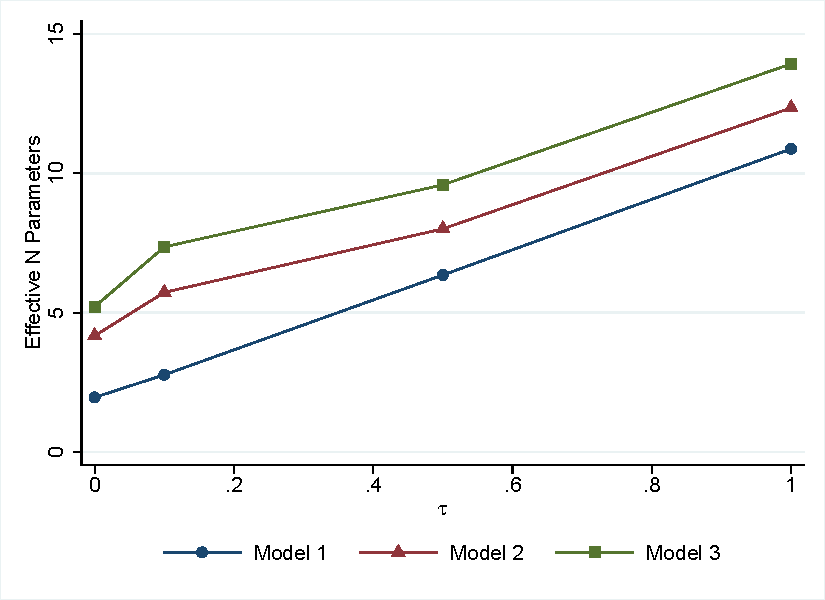
\includegraphics[height=3in, trim = 1mm 1mm 1mm 1mm, clip=true]
	{chapter_2/figs/p_newitems.pdf}
	\caption{Estimated effective number of parameters for models fit to test data consisting of the same persons responding to new items.}
	\label{fig:k-new-items}
\end{figure}

\begin{figure}[tbp]
	\centering
	\includegraphics[height=3.5in, trim = 1mm 1mm 1mm 1mm, clip=true]
	{chapter_2/figs/select_aic2.pdf}
	\caption{Proportion of times each model was selected using AIC with the ``inverted'' models.}
	\label{fig:select-aicitem}
\end{figure}


\section{Discussion}

\comment{Find papers on choosing between LLTMS.}

\comment{(1) K-fold CV. (2) Consider a linear model to parallel holdout CV with new items. Possible to get marginal likelihood with linear model? (3) Show that AIC works with ``De Boeck'' version of model. (4) Consider extending topic to include linear crossed mixed-effects models.}

%\bibliographystyle{apacite}
%\bibliography{../../Documents/References/references}

\end{document}


